\chapter{Object Detection using Computer Vision}

\paragraph*{}
In the current simulation on Webots, the object detection system utilizes OpenCV with a masking method to identify and interact with a yellow object in the arena. The task involves detecting and moving a yellow cylindrical object, randomly placed within the arena, to a specified location.

\paragraph*{}
The detection process commences with the robot utilizing an RGB camera mounted on the front-most part of the TurtleBot3 to capture its surrounding environment. To address potential issues related to the robot's physics and balance, the RGB camera is approximated as a point source, as illustrated in Figure~\ref{fig:object detection figure 1}. The captured image is subsequently converted into the HSV color space to facilitate the segmentation of the yellow object based on a predefined color range. A mask is then applied to the regions containing the yellow color, enabling the generation of a contour around the detected object. This contour functions as a visual boundary, allowing the robot to perceive and localize the object with precision.

\begin{figure}[H]
    \centering
    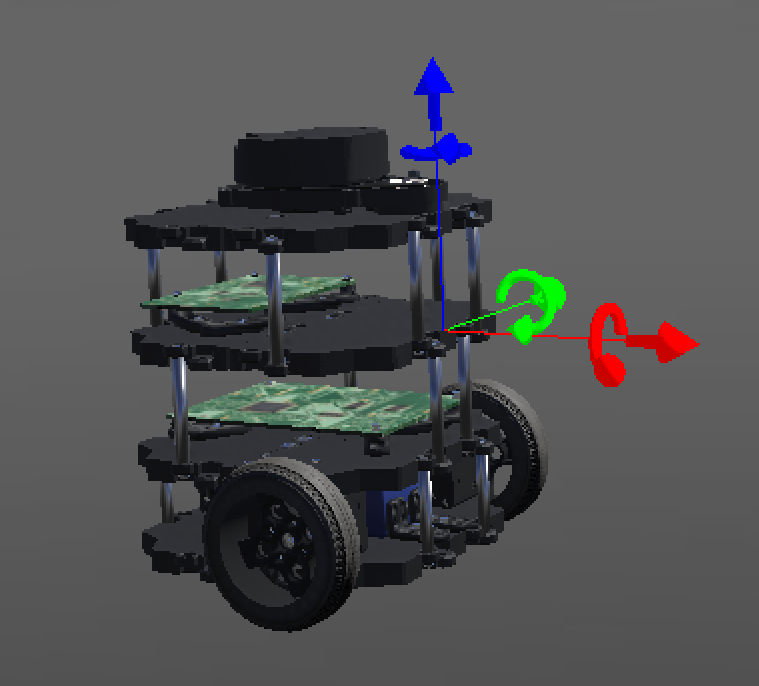
\includegraphics[width=0.5\linewidth]{assets/images/object_detection/fig1.png}
    \caption{The location of the RGB camera mounted on the TurtleBot3}
    \label{fig:object detection figure 1} 
\end{figure}


\paragraph*{}
Once the object is detected, the robot moves until the contour is centered within the camera frame, ensuring that the robot faces the object directly. This alignment is achieved by comparing the distances between the left and right edges of the bounding box surrounding the contour and the corresponding edges of the camera frame. Specifically, the distance between the left edge of the frame and the left edge of the bounding box is compared with the distance between the right edge of the frame and the right edge of the bounding box. The robot stops when the difference between these two distances is less than or equal to 1, as the camera calculates distances as whole numbers. Using a threshold of \(\leq 1\) is more reliable than requiring exact equality, as slight variations in measurement may occur due to the camera's resolution or other factors.

\begin{figure}[H]
    \centering
    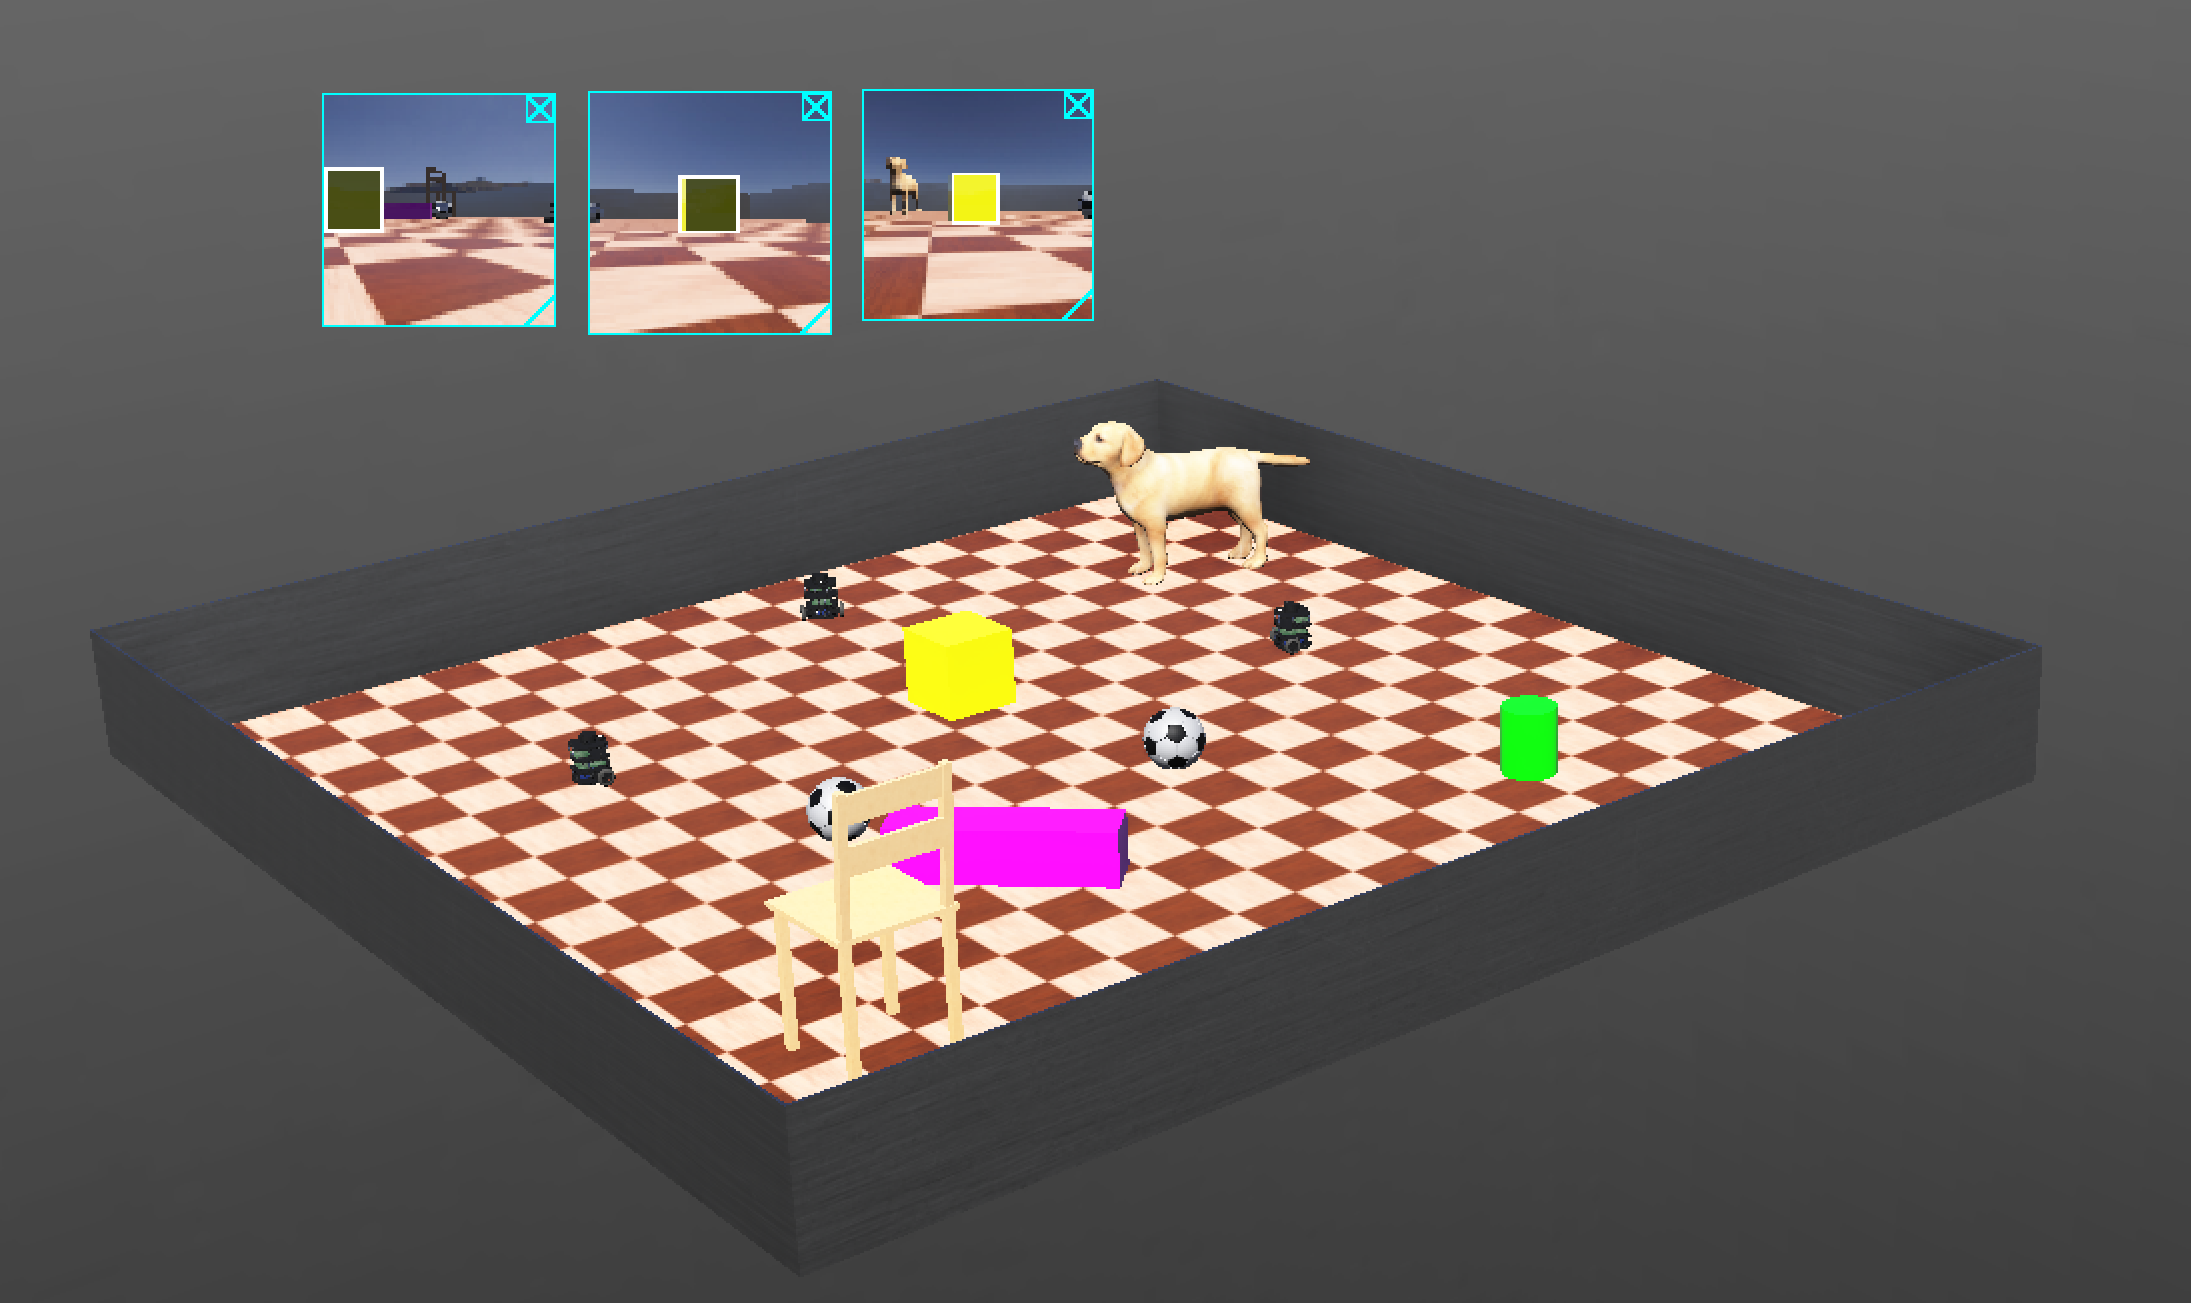
\includegraphics[width=0.7\linewidth]{assets/images/object_detection/fig2.png}
    \caption{The location of the RGB camera mounted on the TurtleBot3}
    \label{fig:object detection figure 2} 
\end{figure}

\paragraph*{}
After aligning with the object as shown in Figure~\ref{fig:object detection figure 2}, the robot calculates the real-world distance from its current position to the object's surface. This is achieved by using a pre-calculated focal length of the camera, derived from the following formulas:

\begin{equation}
\text{f} = \frac{H_{\text{real}}\cdot D_{\text{known}}}{H_{\text{img}}}\
\end{equation}

\begin{equation}
\text d_{\text{real}} = \frac{H_{\text{real}}\cdot f}{H_{\text{img}}}\
\end{equation}

where \(f\) represents the focal length of the camera, \(H_{\text{img}}\) is the known width of the object in the image (in pixels), \(D_{\text{known}}\) denotes the known distance to the object (in meters), \(H_{\text{real}}\) is the real-world width of the object (in meters), and {\text{f}} is the focal length of the camera (in pixels).

\paragraph*{}
By defining the known distance and real-world dimensions of the object in the simulation, the system can compute the real-time distance between the robot's camera and the object's surface. This calculation guides the robot on how far it must travel to reach the yellow cylindrical object.

\paragraph*{}
Several adjustments were made to improve the detection system. Increasing the simulation's luminosity setting from 1 to 1.2 enhanced the brightness, ensuring the environment's colors closely resembled real-world conditions. Consequently, the HSV color range for detecting yellow was refined to \((70, 100, 0)\) to \((90, 255, 255)\), making the detection process more reliable and accurate. These modifications addressed earlier issues with color recognition and bridged the gap between simulated and real-world object detection.

\paragraph*{}
The current system demonstrates reliable detection and interaction with a single yellow object. Looking ahead, the goal is to enable robots to detect and interact with objects of varying geometries and colors. This includes incorporating constraints such as object pose estimation, expanding the system's versatility in real-world applications.

\paragraph*{}
In summary, the object detection system combines effective visual processing techniques with a robust control mechanism, allowing robots to detect, align with, and calculate the distance to a target object. These advancements mark a significant step toward achieving the project's broader objectives.